% -----------------------------------------
% File: Rapport.tex
% 
% Compilation: $ pdflatex rapport.tex
% 
% Amir Ben Slimane & Salah Bennour, 2015
% Polytech Nice Sophia - Computer Sciences
% -----------------------------------------

% Préambule du document
\documentclass[a4paper,11pt]{article}
\usepackage[french]{babel}
\usepackage[utf8]{inputenc}
\usepackage[T1]{fontenc}
\usepackage{graphicx}
\usepackage{enumitem}
\usepackage{moreverb}
\usepackage{amsmath,amsfonts,amssymb}

\usepackage[linesnumbered,ruled,vlined]{algorithm2e}
\raggedbottom

\setlength{\topmargin}{-0.8in}
\setlength{\textheight}{10in}
\setlength{\oddsidemargin}{.125in}
\setlength{\textwidth}{6in}
\setcounter{secnumdepth}{3}



% Corps du document
\begin{document}

\begin{titlepage}
    \begin{center}
        \vspace*{1cm}
        
       	\vfill
       	\Huge
        \textbf{Commande par ordiateur :\\ Estimation récursive de paramètres}

        \vspace{0.3cm}
        \Large
		Amir Ben Slimane \& Salah Bennour         
        

		\vfill
        \vspace{0.8cm}
        

        \Large
        Science Informatique\\
        Polytech Nice-Sophia - France\\
        01-03-2015
        
    \end{center}
\end{titlepage}

	\newpage

	% Table des matières ; nécessite de compiler deux fois de suite
	\tableofcontents

	\newpage

	\section{Introduction}

		\paragraph{}
		Ce projet consiste à estimer la position et la vitesse initiale d'un objet en mouvement rectiligne uniforme à partir d'angles depuis lesquels un observateur l'observe en \« gravitant \» autour.
		Les angles d'observations se font à chaque intervalle de temps. 

		\paragraph{}
		Une première version du projet prend en compte que l'observateur connaît exactement sa position à chaque intervalle de temps. 

		\paragraph{}
		Une deuxième version voit la mesure de sa position entachée de bruit, l'observateur commettra donc des erreurs sur sa position, et donc sur l'estimation de la position et la vitesse initiale du mobile.
	
		\paragraph{}
		Pour se faire, notre simulation se basera sur des méthodes de résolution de systèmes d'équations. Il sera alors possible de faire une estimation assez proche des paramètres initiaux du mobile.

		\begin{figure}[h]
			\centerline{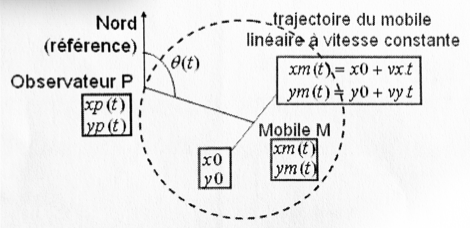
\includegraphics[scale=0.50]{img/intro.png}}
			\caption{Schéma du problème}
			\label{diagramme-composants}
		\end{figure}


	\newpage

	\section{Environnement de travail}

		\subsection{Langage de développement}
		\paragraph{}
		Le langage de développement de ce projet est le JAVA. Ce langage répond parfaitement aux besoins, de par son accésibilité que par l'existence de bibliothèques pour afficher une courbe ou bien manipuler des matrices.
		De plus le JAVA est un langage orienté objets dont les élèves de l'école sont spécialistes.

		\subsection{Bibliothèques}
		\paragraph{}
		Pour la manipulation des matrices, la bibliothèque Jblas a répondu parfaitement à nos attentes grâce à son objet DoubleMatrix qui permet de manipuler des matrices de réels. 

		\paragraph{}
		Concernant l'affichage graphique des trajectoires du mobile et de l'observateur, le projet utilise la bibliothèque JfreeChart qui permet la représentation de courbes sur des axes d'orientation.

		\subsection{Tests}
		\paragraph{}
		Pour garantir la veracité et la robustesse de notre modélisation, des tests ont été effectués pour chacun des algorithmes implémentés. Ces tests ont été réalisés à partir de la bibliothèque JUnit.

		\subsection{Dépendances maven}
		\paragraph{}
		Le projet est un projet maven, les dépendances citées ci-dessus sont donc directement téléchargés depuis maven.


		\newpage

	\section{Mise en place du simulateur}

		\paragraph{}
		Le simulateur du projet permet d'instancier les différents objets pour mener à bien notre estimation des paramètres initiaux du mobile.

		\paragraph{}
		Pour cela, il se charge de créer un objet Mobile et un objet Observateur héritant d'un même objet Point. Ces deux objets représentent respectivement le mobile en mouvement rectiligne uniforme et l'observateur qui gravite autour de ce mobile.

		\paragraph{}
		La classe Resolution contient des algorithmes permettant de résoudre un système d’équations sous la forme d'une équation matricielle.
	
		\paragraph{}
		\begin{figure}[h]
			\centerline{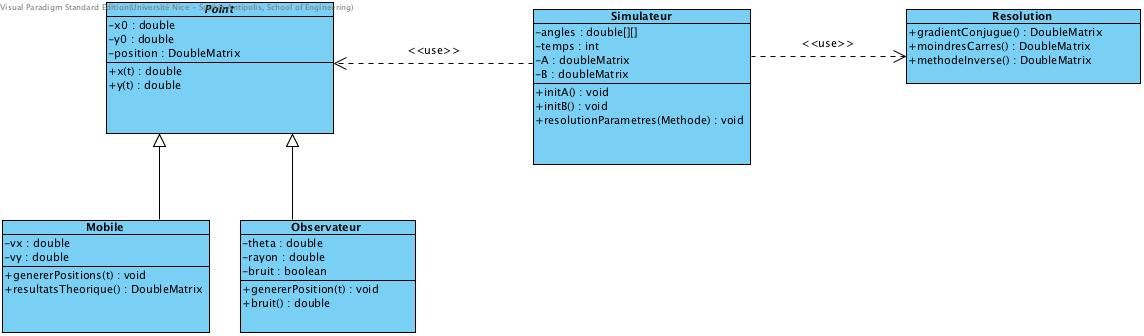
\includegraphics[scale=0.50]{img/diagramme.jpg}}
			\caption{Diagramme de classe}
			\label{diagramme-composants}
		\end{figure}

		\subsection{L'objet Mobile}
		\paragraph{}
		L'objet Mobile est initialisé avec une matrice de taille 2x1 dont les deux valeurs correspondent aux coordonnées initiales du mobile, réspectivement en abscisse et en ordonnée. Un algorithme génère ses positions sur le nombre de périodes souhaitées, la matrice devient alors de taille 2xn. 
		
		\paragraph{}
		Ainsi pour tout t, on a :
	
		\paragraph{}
			\begin{equation} 
				x_{t} = x_{0} + v_{x} \times t 
			\end{equation}
			\begin{equation} 
				y_{t} = y_{0} + v_{y} \times t 
			\end{equation}

 		\begin{itemize}
			\item $x_{t}$ et $y_{t}$ : la position du mobile à un instant t.
			\item $x_{0}$ et $y_{0}$ : la position initiale.
			\item $v_{x}$ et $v_{y}$ : la vitesse
		\end{itemize}

		\newpage

		\subsection{L'observateur}
		\paragraph{}
		Observateur et Mobile héritant de la même classe, le concept de génération des positions reste le même. La génération des positions dépend de la présence ou non du bruit.
		
		\paragraph{}
		Ainsi pour tout t, on a :
		
			\begin{equation} 
				x_{t} = x_{c} + R \times \cos( v \times t) 
			\end{equation}
			\begin{equation} 
				y_{t} = y_{c} + R \times \sin( v \times t) 
			\end{equation}

 		\begin{itemize}
			\item $x_{t}$ et $y_{t}$ : la position du mobile à un instant t.
			\item $x_{c}$ et $y_{c}$ : la position du cercle.
			\item R : le rayon du cercle.
			\item v : la vitesse circulaire.
		\end{itemize}
		
		A ceci, s'ajoute le bruit lorsque la simulation est lancée avec. Le bruit est ici implémenté par la génération d'un nombre aléatoire variant entre [- rayon * 3 \%; rayon * 3 \% ] dont l’espérance mathématique est de 0.

			\begin{equation} 
				x_{t} = x_{c} + R \times \cos( v \times t)  + bruit
			\end{equation}
			\begin{equation} 
				y_{t} = y_{c} + R \times \sin( v \times t) + bruit
			\end{equation}


		\subsection{Le simulateur}
		\paragraph{}
		Le simulateur a pour tache de générer les déplacements de l'observateur et du mobile au cours du temps t. En fonction de ces positions, il calcule alors l'angle qu'il y a entre ces deux objets pour chaque intervalle t. Lors de la prise en compte du bruit, la position de l'observateur n'étant pas exacte, les mesures d'angles se retrouvent être imprécis.

		\paragraph{}
			\begin{equation} 
				angle_{t} = atan2( y_{mobile}(t) -  y_{observateur}(t) , x_{mobile}(t) -  x_{observateur}(t) )
			\end{equation}

		\paragraph{}
		Une fois toutes les générations des positions de l'observateur et du mobile faites, on génère les matrices A et B.
		Pour cela nous utilisons l'erreur de prédiction qui est nulle si les mesures sont parfaites. A chaque intervalle de temps, on doit donc avoir une prédiction nulle.

		\paragraph{}
		L’erreur de prédiction est la suivante :

		\paragraph{}
		\begin{equation}
		   \begin{split}
		      \epsilon=&\cos(\theta(t)) \times y_p(t) -\sin(\theta(t)) \times x_p(t)\\
		        &+\sin(\theta(t)) \times x_0 +\sin(\theta(t)) \times t \times v_x\\
		        &-\cos(\theta(t)) \times y_0 -\cos(\theta(t)) \times t \times v_y
		   \end{split}
		\end{equation}

		\paragraph{}
		Avec $\epsilon=0$ lorsque les mesures sont parfaites.

		\paragraph{}
		Les paramètres initiaux du mobile à estimer sont x0, y0, vx et vy. Ce sont les 4 inconnus que le simulateur va chercher à découvrir. Pour ça, il faut donc n équations à un intervalle de temps différent avec n >= 4 car il faut au moins un systeme de 4 équations pour résoudre un systeme d'équations à 4 inconnues.
		Ce qui donne l'équation matricielle suivante
		A * X = B avec A une matrice de taille 4 x n, X et B deux matrices de taille 4 * 1. 

		\paragraph{}
		Ce qui donne en développant :

		\begin{equation}
				\begin{align*}
				\begin{pmatrix}
					\sin(\theta(1)) & -\cos(\theta(1))  & \sin(\theta(1))\times 1 & -\cos(\theta(1))\times 1  \\
					\vdots & \vdots  & \vdots & \vdots  \\
					\sin(\theta(T))  & -\cos(\theta(T))  &  \sin(\theta(T))\times T  &  -\cos(\theta(T))\times T
				\end{pmatrix}
				\times
				\begin{pmatrix}
				 x_0 \\
				 y_0 \\ 
				 v_x \\
				 v_y 
				\end{pmatrix}
				&= 
				\end{align*}
		\end{equation}
		\begin{equation*}
				\begin{pmatrix}
					\sin(\theta(1)) \times x_p(1) - \cos(\theta(1)) \times y_p(1)  \\
					\vdots \\
					\sin(\theta(T)) \times x_p(T) - \cos(\theta(T)) \times y_p(T)  
				\end{pmatrix}
		\end{equation*}

		\newpage

		\subsection{Les tests}
		\paragraph{}
		Afin que la simulation n'ait pas d'erreur, les algorithmes de résolution de systemes d'équations ont été téstés à partir de la bibliothèque JUnit.
		Avant chaque test, on crée nos matrices A et B à partir d'un exemple proposé par Mr Leroux.

		\begin{figure}[h]
			\centerline{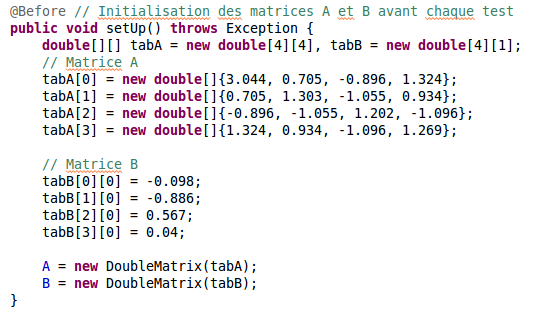
\includegraphics[scale=0.50]{img/testInit.png}}
			\caption{Initialisation des matrices A et B}
			\label{diagramme-composants}
		\end{figure} 

		\paragraph{}
		Une fois nos matrices crées, les differentes méthodes de résolution sont téstées.

		\begin{figure}[h]
			\centerline{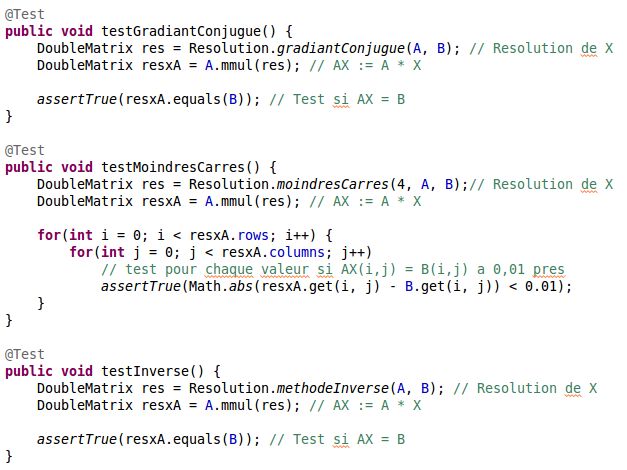
\includegraphics[scale=0.50]{img/testResol.png}}
			\caption{Tests des algorithmes de résolution}
			\label{diagramme-composants}
		\end{figure} 



	\newpage

	\section{Estimation de la vitesse du mobile}
		
		\paragraph{}
		Cette partie du rapport consiste à présenter les différentes méthodes de résolution de l'équation matricielle décrite dans la description du simulateur.

		\paragraph{}
		Pour les exemples, l'objet mobile est initialisé avec les valeurs suivantes :

		\begin{align}
			\begin{pmatrix}
			    x_0 \\
			    y_0 \\
			    v_x \\
			    v_y  
			\end{pmatrix}
			&=
			\begin{pmatrix}
			    10 \\
			    10 \\
			    2 \\
			    2,5
			\end{pmatrix}
		\end{align}

		\subsection{Méthode inverse}

			\subsubsection{Algorithme}

			\paragraph{}
			On peut dès lors utiliser ces deux matrices pour trouver la matrice X en utilisant la formule de la pseudo-inverse.

			\paragraph{}
			En effet d'après l'équation obtenue précédemment, la matrice X est la solution de l'équation linéaire :

			\begin{equation} 
				A^{T} \times A \times X  =  A^{T} \times B
			\end{equation}

			\paragraph{}
			Qui peut également s'écrire en fonction de la pseudo-inverse :

			\begin{equation} 
				X = ( A^{T} \times A)^{-1}  \times  A^{T} \times B
			\end{equation}


			\subsubsection{Implémentation}

			\begin{figure}[h]
				\centerline{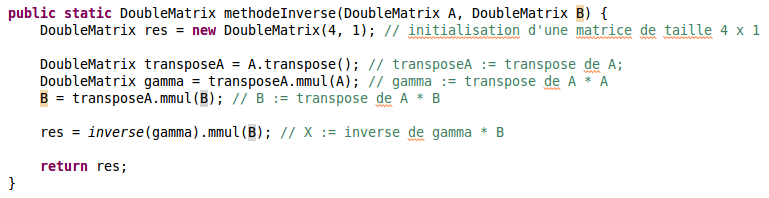
\includegraphics[scale=0.50]{img/inverse.png}}
				\caption{Implémentation de la méthode par l'inverse}
				\label{diagramme-composants}
			\end{figure}


			\subsubsection{Résultats obtenus}

			\begin{table}[h]
			\begin{tabular}{|l|l|l|l|}
			\hline
			\multicolumn{2}{|l|}{Sans bruit} & \multicolumn{2}{l|}{Avec bruit} \\ \hline
			Estimation & Erreur & Estimation & Erreur \\ \hline
						\begin{pmatrix} 10 \\ 10 \\ 2 \\ 2.5	\end{pmatrix}
						&	
						\begin{pmatrix} 2.61E-12 \\ 2.05E-12 \\ 2.70E-13 \\ 1.42E-13\end{pmatrix}       
						&
						\begin{pmatrix} 10 \\ 10 \\ 2\\ 2,5	\end{pmatrix}
			             &     
			 			\begin{pmatrix} 6.25E-13 \\ 1.70E-13 \\ 1.21E-13 \\ 0	\end{pmatrix} \\ \hline
			\end{tabular}
			\end{table}

			\paragraph{}
			Les résultats calculés avec et sans bruit sont excellents. Ils resten relativement bon et assez proche de la réalité.


	\newpage

		\subsection{Méthode du gradient conjugué}

			\subsubsection{Algorithme}

			\paragraph{}
			Toujours à partir des matrices A et B, il est possible de retrouver le résultat grâce à la méthode du gradient conjugué.

			\paragraph{}
			En effet, la méthode du gradient conjugué nous permet de résoudre une équation du même type que celle qui se présente ici, à savoir T \time x = b.


			\paragraph{}
			Pour ce faire, il y'a un algorithme à suivre :

			\begin{figure}[h]
				\centerline{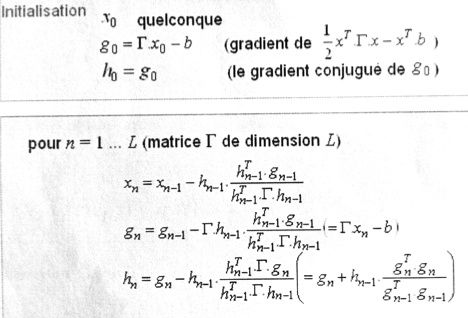
\includegraphics[scale=0.50]{img/gradient_conjugue.png}}
				\caption{Gradient conjugué }
				\label{diagramme-composants}
			\end{figure}

			\subsubsection{Implémentation}

			\begin{figure}[h]
				\centerline{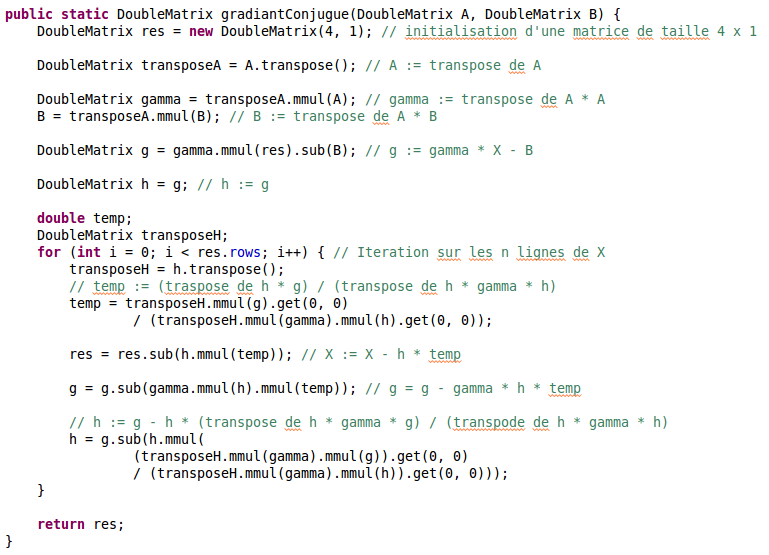
\includegraphics[scale=0.50]{img/gradiantConjugue.png}}
				\caption{Implémentation de la méthode su gradiant conjugué}
				\label{diagramme-composants}
			\end{figure}


			\subsubsection{Résultats obtenus}

			\begin{table}[h]
			\begin{tabular}{|l|l|l|l|}
			\hline
			\multicolumn{2}{|l|}{Sans bruit} & \multicolumn{2}{l|}{Avec bruit} \\ \hline
			Estimation & Erreur & Estimation & Erreur \\ \hline
					\begin{pmatrix} 10 \\ 10 \\ 2 \\ 2.5	\end{pmatrix}
						&	
						\begin{pmatrix} 2.74E-12 \\ 1.82E-11 \\ 5.78E-11 \\ 2.49E-10\end{pmatrix}       
						&
						\begin{pmatrix} 10 \\ 10 \\ 2\\ 2,5	\end{pmatrix}
			             &     
			 			\begin{pmatrix} 4.88E-12 \\ 2.98E-11 \\ 9.85E-11 \\ 4.07E-10\end{pmatrix} \\ \hline
			\end{tabular}
			\end{table}

			\paragraph{}
			Même constat qu’avec la méthode inverse,les résultats obtenus étant assez similaires.

	\newpage

		\subsection{Méthode récursive des moindres carrés}

			\subsubsection{Algorithme}

			\paragraph{}
			Au lieu de disposer d’un vecteur de données et d’effectuer une estimation globale via les méthodes explicitées ci-dessus, les moindres carrés récursifs visent à réactualiser le vecteur des paramètres à chaque nouvelle mesure tout en conservant le même critère.

			\paragraph{}
			L’algorithme à suivre est le suivant :

			\begin{figure}[h]
				\centerline{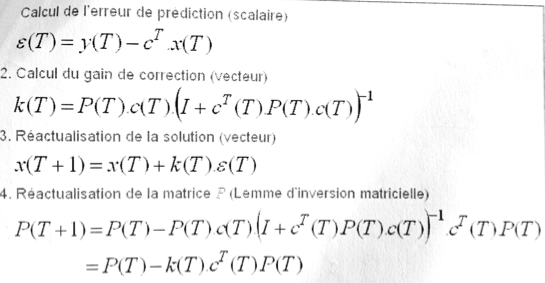
\includegraphics[scale=0.50]{img/moindres_carres_rec.png}}
				\caption{Formule : moindres carrés récursive}
				\label{diagramme-composants}
			\end{figure}

			\subsubsection{Implémentation}

			\begin{figure}[h]
				\centerline{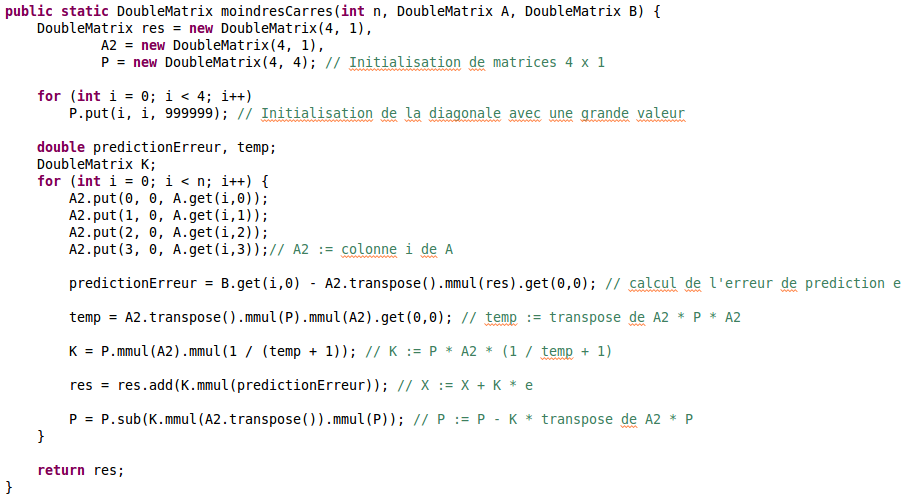
\includegraphics[scale=0.50]{img/moindresCarres.png}}
				\caption{Implémentation de la méthode des moindres carrés}
				\label{diagramme-composants}
			\end{figure}

			\subsubsection{Résultats obtenus}

			\paragraph{}

			\begin{table}[h]
			\begin{tabular}{|l|l|l|l|}
			\hline
			\multicolumn{2}{|l|}{Sans bruit} & \multicolumn{2}{l|}{Avec bruit} \\ \hline
			Estimation & Erreur & Estimation & Erreur \\ \hline
					\begin{pmatrix} 10 \\ 10 \\ 2 \\ 2.5	\end{pmatrix}
						&	
						\begin{pmatrix} 2.62E-5 \\ 2.15E-5 \\ 2.72E-6 \\ 1.91E-6\end{pmatrix}       
						&
						\begin{pmatrix} 10 \\ 10 \\ 2\\ 2,5	\end{pmatrix}
			             &     
			 			\begin{pmatrix} 2.57E-5 \\ 2.09E-5 \\ 2.68E-6 \\ 1.88E-6\end{pmatrix} \\ \hline
			\end{tabular}
			\end{table}

			\paragraph{}
			Dans le cas d'une mesure sans bruit les résultats sont tout aussi bons qu'avec les autres méthodes. Cependant l'éstimation avec bruit nous donne toujours un résultat aussi approximatif.

	\newpage

	\section{Conclusion}
		
		\paragraph{}
		% TODO Quand t'auras finies je ferai ça
		Grâce aux trois méthodes mathématiques présentées ici, il a été possible de déterminer la vitesse et la position initiale du mobile en déplacement. Cependant, aucune des trois méthodes ne s’est réellement démarquée : toutes donnent un résultat plus que correct lorsque la mesure a été effectuée sans bruit, tandis que le résultat reste approximatif – mais tout à fait réaliste – dans le cas d’une mesure avec bruit.

		\paragraph{}
		Dans le cadre du premier projet, il aurait été possible d’intégrer les connaissances acquises ici. En effet, il s’agissait d’un hélicoptère qui devait se poser sur une plateforme non mobile. Il aurait alors été possible de faire bouger cette plateforme, puis d’estimer la position que doit atteindre l’hélicoptère pour atterrir dessus.


\end{document}
